\newpage
\subsection{Exercise 26.7}
\begin{enumerate}
      \begin{multicols}{2}
            \item Water is poured into a container, the relationship between the volume of the
            water and the time is $V = (2t^2 + 3t)$cm$^3$. When $t = 3$s, find the rate of
            change of the volume of the water. \sol{}
            \begin{flalign*}
                  \frac{dV}{dt} & = 4t + 3 &
            \end{flalign*}
            When $t = 3$s,
            \begin{flalign*}
                  \frac{dV}{dt} & = 4(3) + 3 = 15\text{cm}^3/\text{s} &
            \end{flalign*}
            \vfill\null

            \item One throws a piece of stone into the water. The radius of the ripple on the
            water surface caused by the stone is increasing at a rate of $0.1$m/s. When the
            radius is $1$m, find the rate of change of the area of the ripple. \sol{}
            \begin{flalign*}
                  \frac{dr}{dt} & = 0.1\text{m/s}                   & \\
                  A             & = \pi r^2                         & \\
                  \frac{dA}{dr} & = 2\pi r                          & \\
                  \frac{dA}{dt} & = \frac{dA}{dr}\cdot\frac{dr}{dt} & \\
                                & = 2\pi r\cdot 0.1\text{m/s}       & \\
                                & = 0.2\pi r\text{m}^2/\text{s}     &
            \end{flalign*}
            When $r = 1$m,
            \begin{flalign*}
                  \frac{dA}{dt} & = 0.2\pi(1)\text{m}^2/\text{s} \\
                                & = 0.2\pi\text{m}^2/\text{s}
            \end{flalign*}
      \end{multicols}

      \begin{multicols}{2}
            \item The side length of a square is increasing at a rate of $3$cm per second. When
            the side length is $15$cm, find the rate of change of its area. \sol{}
            \begin{flalign*}
                  \frac{ds}{dt} & = 3\text{cm/s}                    & \\
                  A             & = s^2                             & \\
                  \frac{dA}{ds} & = 2s                              & \\
                  \frac{dA}{dt} & = \frac{dA}{ds}\cdot\frac{ds}{dt} & \\
                                & = 2s\cdot 3\text{cm/s}            & \\
                                & = 6s\text{cm}^2/\text{s}          &
            \end{flalign*}
            When $s = 15$,
            \begin{flalign*}
                  \frac{dA}{dt} & = 6(15)\text{cm}^2/\text{s} \\
                                & = 90\text{cm}^2/\text{s}
            \end{flalign*}
            \item A cube expanded after being heated, the rate of change of its side length is
            $5$cm/s. When the side length is $4$cm, find the rate of change of its area.
            \sol{}
            \begin{flalign*}
                  \frac{ds}{dt} & = 5\text{cm/s}                    & \\
                  A             & = 6s^2                            & \\
                  \frac{dA}{ds} & = 12s                             & \\
                  \frac{dA}{dt} & = \frac{dA}{ds}\cdot\frac{ds}{dt} & \\
                                & = 12s\cdot 5\text{cm/s}           & \\
                                & = 60s\text{cm}^2/\text{s}         &
            \end{flalign*}
            When $s = 4$,
            \begin{flalign*}
                  \frac{dA}{dt} & = 60(4)\text{cm}^2/\text{s} \\
                                & = 240\text{cm}^2/\text{s}
            \end{flalign*}
      \end{multicols}

      \newpage
      \item The radius of a sphere increases by 1cm per second. When the radius is 3cm,
            find the rate of change of its volume. \sol{}
            \begin{flalign*}
                  \frac{dr}{dt} & = 1\text{cm/s}                    & \\
                  V             & = \frac{4}{3}\pi r^3              & \\
                  \frac{dV}{dr} & = 4\pi r^2                        & \\
                  \frac{dV}{dt} & = \frac{dV}{dr}\cdot\frac{dr}{dt} & \\
                                & = 4\pi r^2\cdot 1\text{cm/s}      & \\
                                & = 4\pi r^2\text{cm}^3/\text{s}    &
            \end{flalign*}
            When $r = 3$,
            \begin{flalign*}
                  \frac{dV}{dt} & = 4\pi(3)^2\text{cm}^3/\text{s} \\
                                & = 36\pi\text{cm}^3/\text{s}
            \end{flalign*}

      \item The area of a circle increases by 5cm$^2$ per minute. When the circumference of
            the circle is 40cm, find the rate of change of its radius. \sol{}
            \begin{flalign*}
                  \frac{dA}{dt} & = 5\text{cm}^2/\text{min}              & \\
                  A             & = \pi r^2                              & \\
                  \frac{dA}{dr} & = 2\pi r                               & \\
                  \frac{dr}{dt} & = \frac{dr}{dA}\cdot\frac{dA}{dt}      & \\
                                & = \frac{1}{2\pi r}\cdot 5\text{cm}^2   & \\
                                & = \frac{5}{2\pi r}\text{cm}/\text{min} &
            \end{flalign*}
            When $C = 40$,
            \begin{flalign*}
                  2\pi r        & = 40                                                            \\
                  r             & = \dfrac{20}{\pi}                                               \\
                  \frac{dr}{dt} & = \frac{5}{2\pi\left(\frac{20}{\pi}\right)}\text{cm}/\text{min} \\
                                & = \frac{5}{40}\text{cm}/\text{min}                              \\
                                & = \frac{1}{8}\text{cm}/\text{min}
            \end{flalign*}

            \newpage
            \begin{multicols}{2}
                  \item The volume of a sphere decreases at a rate of $12\pi$cm$^3$ per minute. When
                  the radius of the sphere is 6cm, find the rate of change of its radius and
                  surface area. \sol{}
                  \begin{flalign*}
                        \frac{dV}{dt} & = -12\pi\text{cm}^3/\text{min}                               & \\
                        V             & = \frac{4}{3}\pi r^3                                         & \\
                        \frac{dV}{dr} & = 4\pi r^2                                                   & \\
                        \frac{dr}{dt} & = \frac{dr}{dV}\cdot\frac{dV}{dt}                            & \\
                                      & = \frac{1}{4\pi r^2}\cdot(-12\pi\text{cm}^3/\text{min})      & \\
                                      & = -\frac{3}{r^2}\text{cm}/\text{min}                         & \\
                        A             & = 4\pi r^2                                                   & \\
                        \frac{dA}{dr} & = 8\pi r                                                     & \\
                        \frac{dA}{dt} & = \frac{dA}{dr}\cdot\frac{dr}{dt}                            & \\
                                      & = 8\pi r\cdot\left(-\frac{3}{r^2}\text{cm}/\text{min}\right) & \\
                                      & = -\frac{24\pi}{r}\text{cm}^2/\text{min}                     &
                  \end{flalign*}
                  When $r = 6$,
                  \begin{flalign*}
                        \frac{dr}{dt} & = -\frac{3}{(6)^2}\text{cm}/\text{min}   & \\
                                      & = -\frac{1}{12}\text{cm}/\text{min}      & \\
                        \frac{dA}{dt} & = -\frac{24\pi}{6}\text{cm}^2/\text{min} & \\
                                      & = -4\pi\text{cm}^2/\text{min}
                  \end{flalign*}

                  \item The surface area of a sphere increase at a rate of $10$cm$^2$/s. When its
                  radius is 5cm, find the rate of change of its radius and volume. \sol{}
                  \begin{flalign*}
                        \frac{dA}{dt} & = 10\text{cm}^2/\text{s}                                       & \\
                        A             & = 4\pi r^2                                                     & \\
                        \frac{dA}{dr} & = 8\pi r                                                       & \\
                        \frac{dr}{dt} & = \frac{dr}{dA}\cdot\frac{dA}{dt}                              & \\
                                      & = \frac{1}{8\pi r}\cdot 10\text{cm}^2/\text{s}                 & \\
                                      & = \frac{5}{4\pi r}\text{cm}/\text{s}                           & \\
                        V             & = \frac{4}{3}\pi r^3                                           & \\
                        \frac{dV}{dr} & = 4\pi r^2                                                     & \\
                        \frac{dV}{dt} & = \frac{dV}{dr}\cdot\frac{dr}{dt}                              & \\
                                      & = 4\pi r^2\cdot\left(\frac{5}{4\pi r}\text{cm}/\text{s}\right) & \\
                                      & = 5r\text{cm}^3/\text{s}
                  \end{flalign*}
                  When $r = 5$,
                  \begin{flalign*}
                        \frac{dr}{dt} & = \frac{5}{4\pi(5)}\text{cm}/\text{s} & \\
                                      & = \frac{1}{4\pi}\text{cm}/\text{s}    & \\
                        \frac{dV}{dt} & = 5(5)\text{cm}^3/\text{s}            & \\
                                      & = 25\text{cm}^3/\text{s}
                  \end{flalign*}
            \end{multicols}
            \newpage
      \item Water is poured into the cone shaped container as shown in the diagram below,
            the rate of rising of the water surface is $1$cm per second. When the depth of
            the water is $2m$, find the rate of change of the water volume.
            \begin{center}
                  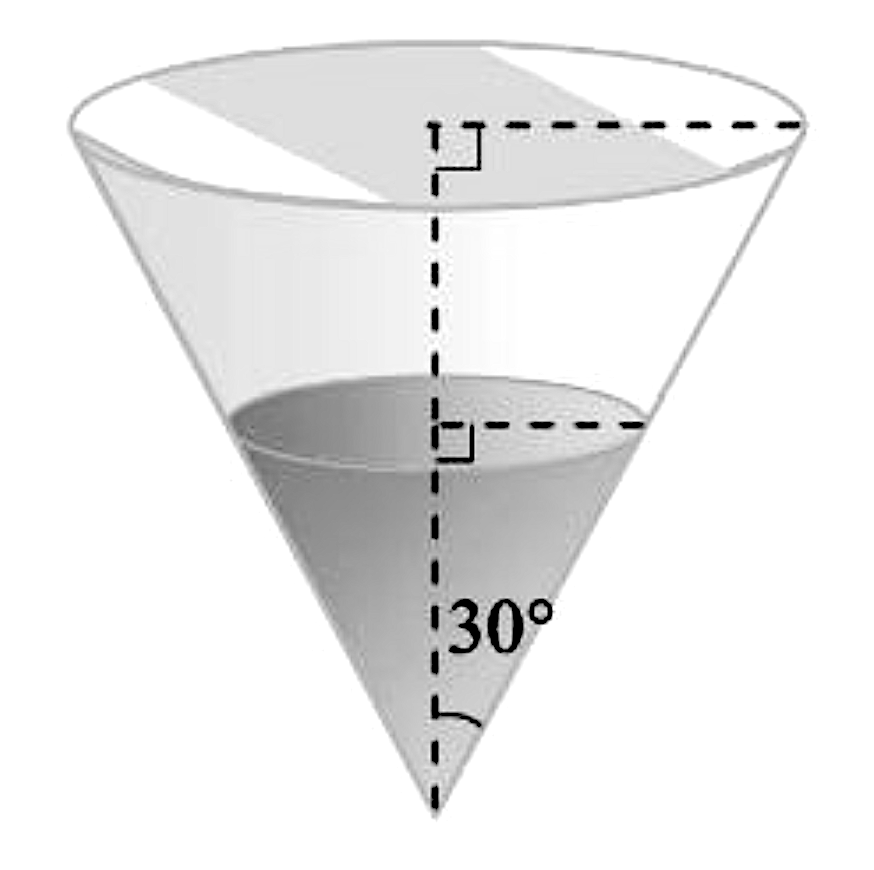
\includegraphics[scale=0.25]{assets/26-15.png}
            \end{center}
            \sol{}
            \begin{flalign*}
                  \dfrac{dh}{dt} & = 1\text{cm/s}                                                           & \\
                  \dfrac{r}{h}   & = \tan 30^\circ = \dfrac{\sqrt{3}}{3}                                    & \\
                  r              & = \dfrac{\sqrt{3}}{3}h                                                   & \\
                  V              & = \dfrac{1}{3}\pi r^2h                                                   & \\
                  \dfrac{dV}{dt} & = \dfrac{1}{3}\pi\left(\dfrac{\sqrt{3}}{3}h\right)^2\text{cm}^3/\text{s} & \\
                                 & = \dfrac{\pi}{9}h^2\text{cm}^3/\text{s}
            \end{flalign*}
            When $h = 2$m $= 200\text{cm}$,
            \begin{flalign*}
                  \dfrac{dV}{dt} & = \dfrac{\pi}{9}(200)^2\text{cm}^3/\text{s} \\
                                 & = \dfrac{40000\pi}{9}\text{cm}^3/\text{s}
            \end{flalign*}

      \item The radius $r$ of a solid cylinder decreases by $0.04$cm per second, its height
            is always equal to 20cm. When the radius is 2cm, find the rate of change of the
            surface area of the cylinder. \sol{}
            \begin{flalign*}
                  \dfrac{dr}{dt} & = -0.04\text{cm/s}                          & \\
                  h              & = 20\text{cm}                               & \\
                  A              & = 2\pi rh + 2\pi r^2                        & \\
                                 & = 40\pi r + 2\pi r^2                        & \\
                  \dfrac{dA}{dr} & = 40\pi + 4\pi r                            & \\
                  \dfrac{dA}{dt} & = \dfrac{dA}{dr}\cdot\dfrac{dr}{dt}         & \\
                                 & = (40\pi + 4\pi r)\cdot(-0.04\text{cm/s})   & \\
                                 & = (-1.6\pi - 0.16\pi r)\text{cm}^2/\text{s} &
            \end{flalign*}
            \vspace{-0.2cm}
            When $r = 2$,
            \begin{flalign*}
                  \dfrac{dA}{dt} & = (-1.6\pi - 0.16\pi(2))\text{cm}^2/\text{s} \\
                                 & = -2.92\pi\text{cm}^2/\text{s}
            \end{flalign*}

      \item Given the function $y = x^3 + 10$. When the rate of change of $y$ is 27 times
            the rate of change of $x$, find the value of $x$. \sol{}
            \begin{flalign*}
                  \dfrac{dy}{dx} & = 3x^2  & \\
                  dy             & = 27dx  & \\
                  \dfrac{dy}{dx} & = 27    & \\
                  3x^2           & = 27    & \\
                  x              & = \pm 3
            \end{flalign*}

      \item Water is poured into a cone shaped container facing downwards with a height of
            18m and a base radius of 24m with a speed of 2m$^3$ per minute. When the height
            of the water is 6m, find the rate of rising of the water surface. \sol{}
            \begin{flalign*}
                  \dfrac{dV}{dt} & = 2\text{m}^3/\text{min}                                               & \\
                  \dfrac{18}{h}  & = \dfrac{24}{r}                                                        & \\
                  r              & = \dfrac{4}{3}h                                                        & \\
                  V              & = \dfrac{1}{3}\pi r^2h                                                 & \\
                                 & = \dfrac{1}{3}\pi\left(\dfrac{4}{3}h\right)^2h                         & \\
                                 & = \dfrac{16\pi}{9}h^3\text{m}^3                                        & \\
                  \dfrac{dV}{dh} & = \dfrac{16\pi}{9}h^2\text{m}^3                                        & \\
                  \dfrac{dh}{dt} & = \dfrac{dh}{dV}\cdot\dfrac{dV}{dt}                                    & \\
                                 & = \dfrac{1}{\dfrac{16\pi}{9}h^2\text{m}^3}\cdot 2\text{m}^3/\text{min} & \\
                                 & = \dfrac{9}{8\pi h^2}\text{m}/\text{min}                               &
            \end{flalign*}
            When $h = 6$m,
            \begin{flalign*}
                  \dfrac{dh}{dt} & = \dfrac{9}{8\pi(6)^2}\text{m}/\text{min} \\
                                 & = \dfrac{9}{288\pi}\text{m}/\text{min}    \\
                                 & = \dfrac{1}{32\pi}\text{m}/\text{min}
            \end{flalign*}
\end{enumerate}
\newpage